\documentclass[]{article}
\usepackage{lmodern}
\usepackage{amssymb,amsmath}
\usepackage{ifxetex,ifluatex}
\usepackage{fixltx2e} % provides \textsubscript
\ifnum 0\ifxetex 1\fi\ifluatex 1\fi=0 % if pdftex
  \usepackage[T1]{fontenc}
  \usepackage[utf8]{inputenc}
\else % if luatex or xelatex
  \ifxetex
    \usepackage{mathspec}
    \usepackage{xltxtra,xunicode}
  \else
    \usepackage{fontspec}
  \fi
  \defaultfontfeatures{Mapping=tex-text,Scale=MatchLowercase}
  \newcommand{\euro}{€}
\fi
% use upquote if available, for straight quotes in verbatim environments
\IfFileExists{upquote.sty}{\usepackage{upquote}}{}
% use microtype if available
\IfFileExists{microtype.sty}{%
\usepackage{microtype}
\UseMicrotypeSet[protrusion]{basicmath} % disable protrusion for tt fonts
}{}
\usepackage[margin=1in]{geometry}
\usepackage{color}
\usepackage{fancyvrb}
\newcommand{\VerbBar}{|}
\newcommand{\VERB}{\Verb[commandchars=\\\{\}]}
\DefineVerbatimEnvironment{Highlighting}{Verbatim}{commandchars=\\\{\}}
% Add ',fontsize=\small' for more characters per line
\usepackage{framed}
\definecolor{shadecolor}{RGB}{248,248,248}
\newenvironment{Shaded}{\begin{snugshade}}{\end{snugshade}}
\newcommand{\KeywordTok}[1]{\textcolor[rgb]{0.13,0.29,0.53}{\textbf{{#1}}}}
\newcommand{\DataTypeTok}[1]{\textcolor[rgb]{0.13,0.29,0.53}{{#1}}}
\newcommand{\DecValTok}[1]{\textcolor[rgb]{0.00,0.00,0.81}{{#1}}}
\newcommand{\BaseNTok}[1]{\textcolor[rgb]{0.00,0.00,0.81}{{#1}}}
\newcommand{\FloatTok}[1]{\textcolor[rgb]{0.00,0.00,0.81}{{#1}}}
\newcommand{\CharTok}[1]{\textcolor[rgb]{0.31,0.60,0.02}{{#1}}}
\newcommand{\StringTok}[1]{\textcolor[rgb]{0.31,0.60,0.02}{{#1}}}
\newcommand{\CommentTok}[1]{\textcolor[rgb]{0.56,0.35,0.01}{\textit{{#1}}}}
\newcommand{\OtherTok}[1]{\textcolor[rgb]{0.56,0.35,0.01}{{#1}}}
\newcommand{\AlertTok}[1]{\textcolor[rgb]{0.94,0.16,0.16}{{#1}}}
\newcommand{\FunctionTok}[1]{\textcolor[rgb]{0.00,0.00,0.00}{{#1}}}
\newcommand{\RegionMarkerTok}[1]{{#1}}
\newcommand{\ErrorTok}[1]{\textbf{{#1}}}
\newcommand{\NormalTok}[1]{{#1}}
\usepackage{longtable,booktabs}
\usepackage{graphicx}
\makeatletter
\def\maxwidth{\ifdim\Gin@nat@width>\linewidth\linewidth\else\Gin@nat@width\fi}
\def\maxheight{\ifdim\Gin@nat@height>\textheight\textheight\else\Gin@nat@height\fi}
\makeatother
% Scale images if necessary, so that they will not overflow the page
% margins by default, and it is still possible to overwrite the defaults
% using explicit options in \includegraphics[width, height, ...]{}
\setkeys{Gin}{width=\maxwidth,height=\maxheight,keepaspectratio}
\ifxetex
  \usepackage[setpagesize=false, % page size defined by xetex
              unicode=false, % unicode breaks when used with xetex
              xetex]{hyperref}
\else
  \usepackage[unicode=true]{hyperref}
\fi
\hypersetup{breaklinks=true,
            bookmarks=true,
            pdfauthor={Andrea García Tapia, Andrea Frenández , Mario Becerra},
            pdftitle={Algoritmos de Gran Escala},
            colorlinks=true,
            citecolor=blue,
            urlcolor=blue,
            linkcolor=magenta,
            pdfborder={0 0 0}}
\urlstyle{same}  % don't use monospace font for urls
\setlength{\parindent}{0pt}
\setlength{\parskip}{6pt plus 2pt minus 1pt}
\setlength{\emergencystretch}{3em}  % prevent overfull lines
\setcounter{secnumdepth}{5}

%%% Use protect on footnotes to avoid problems with footnotes in titles
\let\rmarkdownfootnote\footnote%
\def\footnote{\protect\rmarkdownfootnote}

%%% Change title format to be more compact
\usepackage{titling}
\setlength{\droptitle}{-2em}
  \title{Algoritmos de Gran Escala}
  \pretitle{\vspace{\droptitle}\centering\huge}
  \posttitle{\par}
  \author{Andrea García Tapia, Andrea Frenández , Mario Becerra}
  \preauthor{\centering\large\emph}
  \postauthor{\par}
  \predate{\centering\large\emph}
  \postdate{\par}
  \date{24 de mayo de 2015}


\usepackage{float}
\usepackage{morefloats}
\usepackage[spanish]{babel}
\usepackage{graphicx}
\usepackage{tcolorbox}
\usepackage{rotating}
\usepackage{longtable}
\usepackage{colortbl}
%\usepackage{natbib}
%\newenvironment{scaleb}{ \scalebox{0.4}{} {} }
%\newenvironment{scaleb}{ \tiny{} }
% biber
\usepackage[autostyle]{csquotes}

\usepackage[
    backend=biber,
    style=authoryear-icomp,
    sortlocale=de_DE,
    natbib=true,
    url=false,
    doi=true,
    eprint=false
]{biblatex}
\addbibresource{bibliografia.bib}

\usepackage[]{hyperref}
\hypersetup{
% Turn on this if you prefer to have links colored instead of marked with squares
colorlinks = true,
linkcolor = black,
urlcolor = blue,
citecolor = black,
% pdfpagemode = UseNone
}

\renewcommand\figurename{Figura}
\renewcommand\tablename{Tabla}

\newenvironment{myexampleblock}[1]{%
    \tcolorbox[beamer,%
    noparskip,breakable,
    colback=LightGreen,colframe=DarkGreen,%
    colbacklower=LimeGreen!75!LightGreen,%
    title=#1]}%
    {\endtcolorbox}

\newenvironment{myalertblock}[1]{%
    \tcolorbox[beamer,%
    noparskip,breakable,
    colback=LightCoral,colframe=DarkRed,%
    colbacklower=Tomato!75!LightCoral,%
    title=#1]}%
    {\endtcolorbox}

\newenvironment{myblock}[1]{%
    \tcolorbox[beamer,%
    noparskip,breakable,
    colback=LightBlue,colframe=DarkBlue,%
    colbacklower=DarkBlue!75!LightBlue,%
    title=#1]}%
    {\endtcolorbox}


\begin{document}

\maketitle


{
\hypersetup{linkcolor=black}
\setcounter{tocdepth}{2}
\tableofcontents
}
\pagebreak

\section{Análisis Exploratorio de
Datos}\label{analisis-exploratorio-de-datos}

México ha tenido un incremento en los costos económicos de desastres
asociados a fenómenos hidrometeorológicos, huracanes e inundaciones,
entre otros. En 2010 se presentaron las mayores pérdidas económicas en
la historia del país por fenómenos hidrometeorológicos y geológicos; en
total se perdió el 0.8\% del PIB y se estima que, una vez calculado en
su totalidad, el daño por las tormentas tropicales Ingrid y Manuel en
2013 supere los valores anteriores.

Una pregunta clave que todavía no se contesta en México es si este
incremento en daños y pérdidas se debe a un cambio en la distribución de
los desastres o a observaciones atípicas. El Sistema de Protección Civil
(SINAPROC) define desastre ``al resultado de la ocurrencia de uno o más
agentes perturbadores severos y o extremos, concatenados o no, de origen
natural o de la actividad humana, que cuando acontecen en un tiempo y en
una zona determinada, causan daños y que por su magnitud exceden la
capacidad de respuesta de la comunidad afectada''; sin embargo no esta
definida qué es la capacidad de respuesta de la comunidad afectada ni
existen indicadores. Nuestro sistema es reactivo y las reglas de
operación no son muy claras. EL Panel Intergubernamental de Cambio
Climático (IPCC) prevee un aumento en la frecuencia e intensidad de los
desastres hidrometeoroógicos debido al cambio climático.

Actualmente el SINAPROC funciona de la siguiente manera: cuando ocurre
un desastre el Gobierno Estatal solicita una evaluación al Gobierno
Federal. Este a su vez solicita al Servicio Meteorológico Nacional
(SMN), al Sismológico, Comisión Nacional Forestal (CONAFOR) o al Centro
Nacional de Prevención de Desastres (CENAPRED), dependiendo el tipo de
desastre, la corroboración del evento. Una vez corroborado el Gobierno
Federal decide si lo declara o no . Si lo declara tiene tres opciones:
Contingencia Climática, Desastre, Emergencia o una combinación de las
últimas dos. Esta declaratoria hace toda la diferencia ya que si no es
declarado, el evento solo recibe ayuda de protección civil local. Por el
contario si lo declaran desastre (contingencia climatica, desastre o
emergencia) se activa el programa de reconstrucción del FONDEN, el
programa de apoyos de SAGARPA (CADENA) y diversos programas de apoyo
social como el programa de Empleo Temporal de SEDESOL. Es por ello que
es tan importante tener reglas claras. Este proyecto busca clarificar
las reglas del proceso de declaratoria de desastres naturales y
encontrar un modelo que ayude al Gobierno Federal acelerar los procesos
de decalratoria, ya que actuar de manera oportuna es vital.

Los datos fueron obtenidos del Centro Nacional de Prevención de
Desastres (CENAPRED) para los desastres Hidrometeorológicos de
2000-2010. La base se llama Impacto Socio Económico y es con la que
realizan la serie anual de los libros con el mismo nombre. Se unió con
la base Marginación de CONEVAL y con una base de Riesgos realizada por
el Centro Mario Molina (CMM). La base de Riesgos fue realizada para 5
peligros (huracán, inundación, sequía, incendio forestal, deslave)
calculados a partir de las características geofísicas del país y las
tasas de retorno de los desastres.

\subsection{Descripción del Dataset}\label{descripcion-del-dataset}

La base se conforma de 25 variables, entre las cuales hay
características geográficas (riesgos), características socioeconómicas
de la población y características del evento.

\begin{figure}[H]
\centering
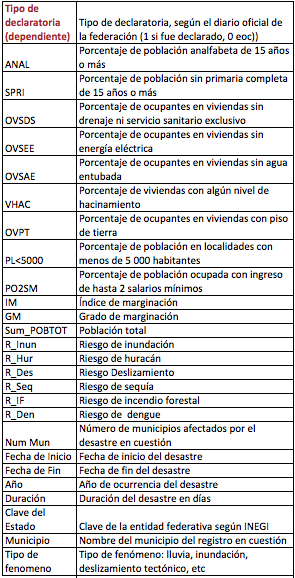
\includegraphics[width=0.45\textwidth]{img/var.png}
\caption{Descripción de variables en la base de datos.}

\end{figure}

Se dividió el conjunto de datos (4750 observaciones con 25 variables) en
datos de entrenamiento (70\%) y de prueba (30\%). La distribución por
Grado de Marginación nos muestra que los grados altos tienen mas
declaratorias.

\begin{figure}[H]
\centering
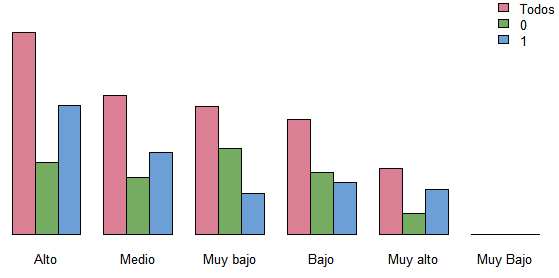
\includegraphics[width=0.8\textwidth]{img/dec_GM.png}
\caption{Distribución por grado de marginación.}

\end{figure}

En cuanto al tipo de fenómeno la mayor parte de las declaratorias se
concentran en lluvias y sequías.

\begin{figure}[H]
\centering
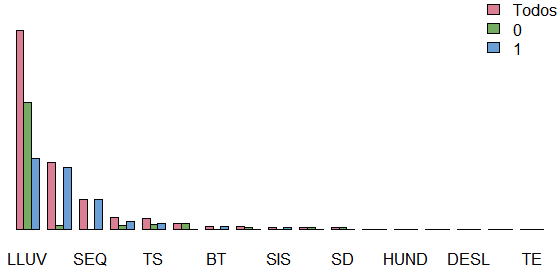
\includegraphics[width=0.8\textwidth]{img/tipo.png}
\caption{Distribución por tipo de fenómeno.}

\end{figure}

\begin{figure}[htbp]
\centering
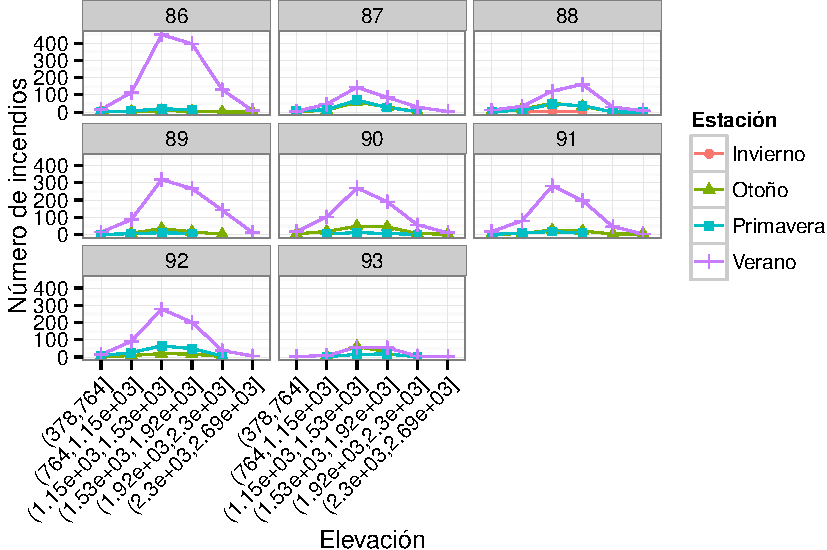
\includegraphics{reporte_files/figure-latex/unnamed-chunk-4-1.pdf}
\caption{Municipios con desastres.}
\end{figure}

\section{Modelos de clasificación}\label{modelos-de-clasificacion}

A continuación se presentan los resultados de los dos clasificadores
utilizados para los datos: regresión logística regularizada y máquina de
soporte vectorial.

\subsection{Regresión Logística
Regularizada}\label{regresion-logistica-regularizada}

Se utilizó el método de \emph{elastic net}, que es una regresión
logística con más parámetros de regularización. Estos parámetros se
escogen a través de validación cruzada.

\begin{longtable}[c]{@{}lrr@{}}
\toprule\addlinespace
& 0 & 1
\\\addlinespace
\midrule\endhead
0 & 254 & 158
\\\addlinespace
1 & 354 & 592
\\\addlinespace
\bottomrule
\addlinespace
\caption{Matriz de confusión de regresión logística}
\end{longtable}

\begin{longtable}[c]{@{}lr@{}}
\toprule\addlinespace
& cm\$byClass
\\\addlinespace
\midrule\endhead
Sensitivity & 0.4177632
\\\addlinespace
Specificity & 0.7893333
\\\addlinespace
Pos Pred Value & 0.6165049
\\\addlinespace
Neg Pred Value & 0.6257928
\\\addlinespace
Prevalence & 0.4477172
\\\addlinespace
Detection Rate & 0.1870398
\\\addlinespace
Detection Prevalence & 0.3033873
\\\addlinespace
Balanced Accuracy & 0.6035482
\\\addlinespace
\bottomrule
\addlinespace
\caption{Evaluación del modelo con regresión logística.}
\end{longtable}

La tasa de clasificación de incorrectos fue de 0.38, la matriz de
confusión se puede ver en el cuadro 4.

\pagebreak 

\subsection{Máquina de Soporte Vectorial en
Paralelo}\label{maquina-de-soporte-vectorial-en-paralelo}

\begin{verbatim}
## [1] "intercepto"
## [1] 0.09747292419257945
\end{verbatim}

\begin{longtable}[c]{@{}lrr@{}}
\toprule\addlinespace
& -1 & 1
\\\addlinespace
\midrule\endhead
-1 & 312 & 194
\\\addlinespace
1 & 296 & 556
\\\addlinespace
\bottomrule
\addlinespace
\caption{Matriz de confusión de SVM}
\end{longtable}

Generamos las métricas con las que se evalúa el desempeño de la
regresión logística pero para el SVM.

\begin{longtable}[c]{@{}lr@{}}
\toprule\addlinespace
& cm2\$byClass
\\\addlinespace
\midrule\endhead
Sensitivity & 0.5131578947368421
\\\addlinespace
Specificity & 0.7413333333333333
\\\addlinespace
Pos Pred Value & 0.6166007905138340
\\\addlinespace
Neg Pred Value & 0.6525821596244131
\\\addlinespace
Prevalence & 0.4477172312223859
\\\addlinespace
Detection Rate & 0.2297496318114874
\\\addlinespace
Detection Prevalence & 0.3726067746686304
\\\addlinespace
Balanced Accuracy & 0.6272456140350877
\\\addlinespace
\bottomrule
\addlinespace
\caption{Evaluación del modelo con SVM.}
\end{longtable}

Se modificó el código pseudodistribuido de la MSV de manera que se
capturara la información de monitoreo del método y fuera posible
explorarla.

\begin{figure}[htbp]
\centering
\includegraphics{reporte_files/figure-latex/unnamed-chunk-10-1.pdf}
\caption{Iteraciones y el número de condición.}
\end{figure}

Los resultados de clasificación con la máquina de soporte vectorial
fueron mejores que con la regresión logística regularizada. La tasa de
clasificación fue menor.

\pagebreak 

\section{Problemas}\label{problemas}

Durante la elaboración de este proyecto nos enfrentamos a diversos
problemas.

\subsection{Implementación del
Cluster}\label{implementacion-del-cluster}

No entendíamos cómo funcionaba el NFS server:

\begin{itemize}
\itemsep1pt\parskip0pt\parsep0pt
\item
  Al utilizar dos carpetas con nombres distintos, es decir
  \texttt{mirrorNFS} y \texttt{carpetaNodo}, no sabíamos que era
  necesario cerrar el loop y correr \texttt{mpirun} en el master desde
  \texttt{carpetaNodo}.
\item
  Cuando intentamos tener un cluster en nuestras computadoras, con las
  diferentes versiones y distribuciones de Linux y una computadora MAC,
  había muchos errores.
\item
  La versión de MPI se actualizó mientras hacíamos las tareas y con un
  \texttt{update} tuvimos que desinstalar y reinstalar todo de nuevo.
\item
  En realidad, todos los problemas por el NFS se solucionaron cuando
  entendimos que éste era solamente una manera de pegarle al master los
  esclavos pero que master siempre considera que está corriendo todo en
  sus versiones.
\end{itemize}

Compilación de archivos:

\begin{itemize}
\itemsep1pt\parskip0pt\parsep0pt
\item
  Las librerías de Lapack, ATLAS, BLAS y las librerías de matemáticas no
  se cargan en \texttt{mpicc} automáticamente para la distribución de
  Linux que usamos (Ubuntu, 14.04, unity). Nos tardamos mucho en
  entender los mensajes de compilación.
\item
  En general, aprender a utilizar \texttt{c} para adaptar los códigos en
  la tarea 3 fue muy problemático.
\end{itemize}

\subsection{Paralelización de SVM}\label{paralelizacion-de-svm}

\begin{itemize}
\itemsep1pt\parskip0pt\parsep0pt
\item
  Nos pasó lo mismo que con \texttt{mpi}: la versión y localización de
  \texttt{R} en \texttt{master} y en cada uno de los \texttt{nodos} debe
  ser exactamente la misma para todas las computadoras en el cluster.
\item
  La instalación de \texttt{rmpi} es muy problemática. Debes de
  realizar\footnote{Gracias al equipo de Liliana, Gabriel y David.}:
\end{itemize}

\begin{verbatim}
sudo apt-get install libcr-dev mpich2 mpich2-doc
R
install.packages('Rmpi')
install.packages('snow')
\end{verbatim}

\begin{itemize}
\itemsep1pt\parskip0pt\parsep0pt
\item
  Primero, intentamos con \texttt{Rmpi}. Sin embargo, fue muy difícil
  debuggear e intentar paralelizar el proceso. Lo que nos pasaba es que
  podíamos prender el cluster en el master pero freezeaba. Cuando leimos
  diferentes foros de ayuda, resultó que este es uno de los errores más
  comunes pero puede tener muchas causas. Eventualmente, al poner la
  bandera de \texttt{manual=T} en el comando para iniciar el cluster, si
  se podía pero teníamos que ir a cada nodo y ejecutar el
  \texttt{script} de \texttt{R} generado en cada uno. Esto no escala.
\item
  Después, logramos correrlo en mpi. Sin embargo, no sabíamos porqué
  estaba repitiendose el proceso tantas veces como procesadores
  teníamos.
\end{itemize}

\begin{figure}[H]
\centering
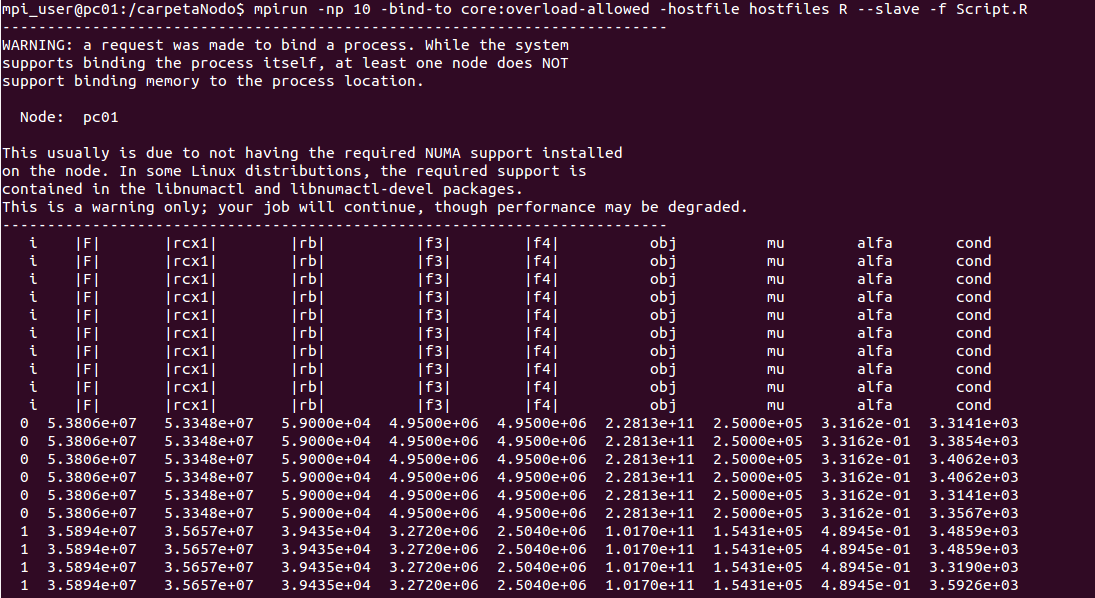
\includegraphics[width=0.8\textwidth]{img/svm_paralelo_mal_p1.png}

\end{figure}

\begin{figure}[H]
\centering
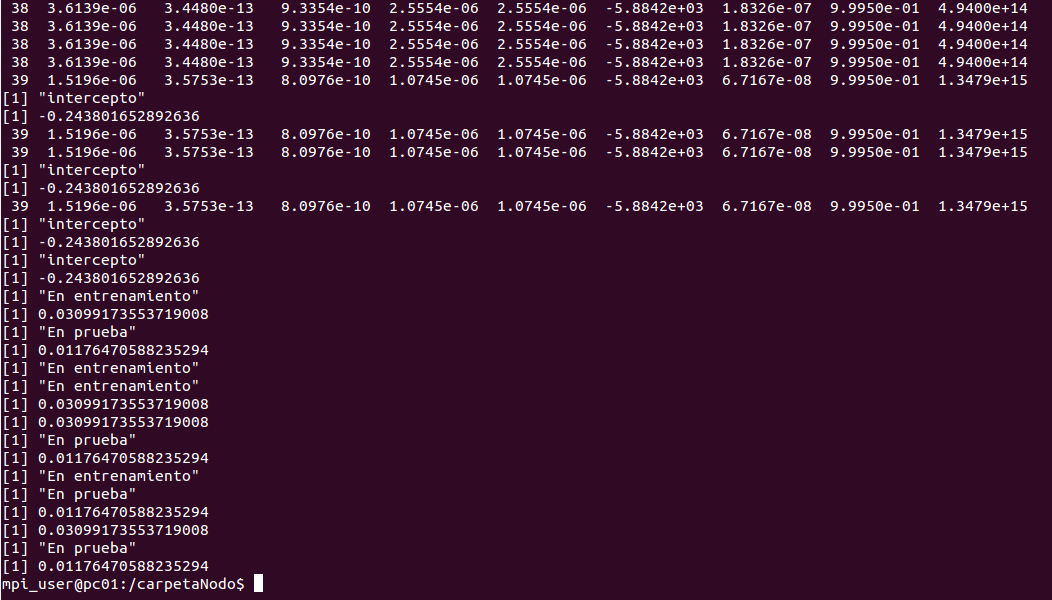
\includegraphics[width=0.8\textwidth]{img/svm_paralelo_mal_p2.png}

\end{figure}

\begin{itemize}
\item
  Probamos muchísimas cosas y nada funcionaba. Entonces, decidimos mejor
  tirar a la basura y cambiar de estrategia.
\item
  Lo que nos funcionó mejor fue utilizar \texttt{snow} directo y mejor
  controlar el cluster desde ahí. Un ejemplo funcional para prenderlo de
  manera interactiva fue (con una sesión en R en \texttt{carpetaNodo} en
  el master):
\end{itemize}

\begin{Shaded}
\begin{Highlighting}[]
\KeywordTok{library}\NormalTok{(snow)}
\CommentTok{# Prendes el cluster}
\NormalTok{cl <-}\StringTok{ }\KeywordTok{makeSOCKcluster}\NormalTok{(}\KeywordTok{c}\NormalTok{(}\StringTok{"slave05"}\NormalTok{,}\StringTok{"localhost"}\NormalTok{))}
\CommentTok{# clusterApply funciona como apply pero mandas el objeto cluster, }
\CommentTok{# x *para iterar*, la funcion(suma, para ejemplificar) y parametros adicionales}
\KeywordTok{clusterApply}\NormalTok{(cl, }\DecValTok{1}\NormalTok{:}\DecValTok{2}\NormalTok{, }\KeywordTok{get}\NormalTok{(}\StringTok{"+"}\NormalTok{), }\DecValTok{3}\NormalTok{)}
\CommentTok{# clusterEvalQ permite enviar comandos a ejecutar en cada nodo para la }
\CommentTok{# sesion de R abierta en cada uno}
\KeywordTok{clusterEvalQ}\NormalTok{(cl, }\KeywordTok{library}\NormalTok{(boot))}
\CommentTok{# detenemos el cluster}
\KeywordTok{stopCluster}\NormalTok{(cl)}
\end{Highlighting}
\end{Shaded}

\begin{itemize}
\itemsep1pt\parskip0pt\parsep0pt
\item
  Para poder conectar bien snow, el único cambio que hay que realizar es
  completar la conexión de dos vías entre master y esclavos, es decir,
  que todos vean a todos con el mismo alias. Por ejemplo, en la master
  (pc01) y en el esclavo (pc05):
\end{itemize}

\begin{figure}[H]
\centering
\includegraphics[width=0.4\textwidth]{img/snow_connectionpc01.png}
\caption{\emph{/etc/hosts} en PC01.}

\end{figure}

\begin{figure}[H]
\centering
\includegraphics[width=0.4\textwidth]{img/snow_connectionpc05.png}
\caption{\emph{/etc/hosts} en PC05.}

\end{figure}

\begin{itemize}
\itemsep1pt\parskip0pt\parsep0pt
\item
  Esta forma nos permitió dejar de utilizar \texttt{mpirun} y poder
  manipular el cluster desde \texttt{R}. Por esto, al final el llamado a
  svm en paralelo es vía \texttt{Rscript}, desde el master y en
  \texttt{carpetaNodo}:
\end{itemize}

\begin{verbatim}
Rscript Script.R
\end{verbatim}

Los resultados se muestran a continuación

\begin{figure}[H]
\centering
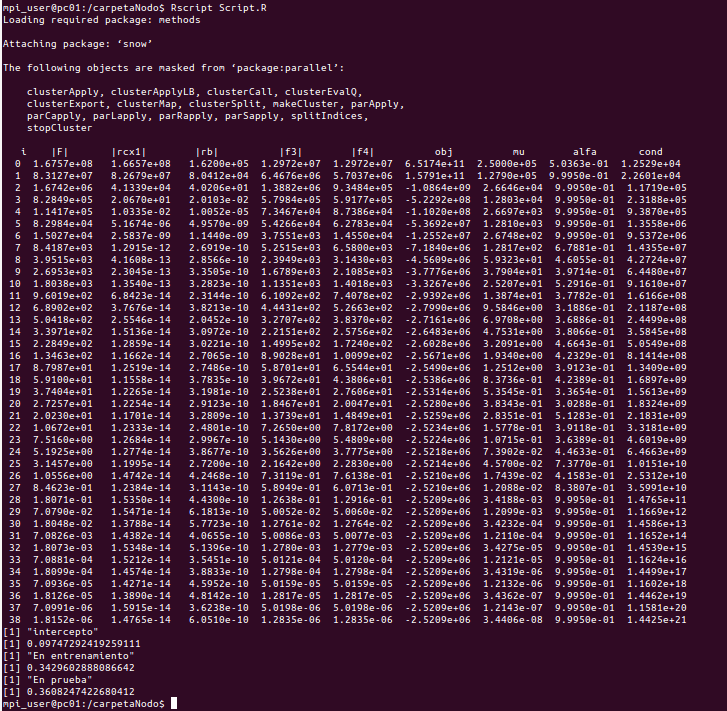
\includegraphics[width=0.8\textwidth]{img/svm_paralelo_bien.png}
\caption{\emph{STOUT} en PC01 de SVM en paralelo.}

\end{figure}

Para revisar que el trabajo se estaba realizando en master y en nodos,
prendimos un \texttt{htop} en el master y el esclavo:

\begin{figure}[H]
\centering
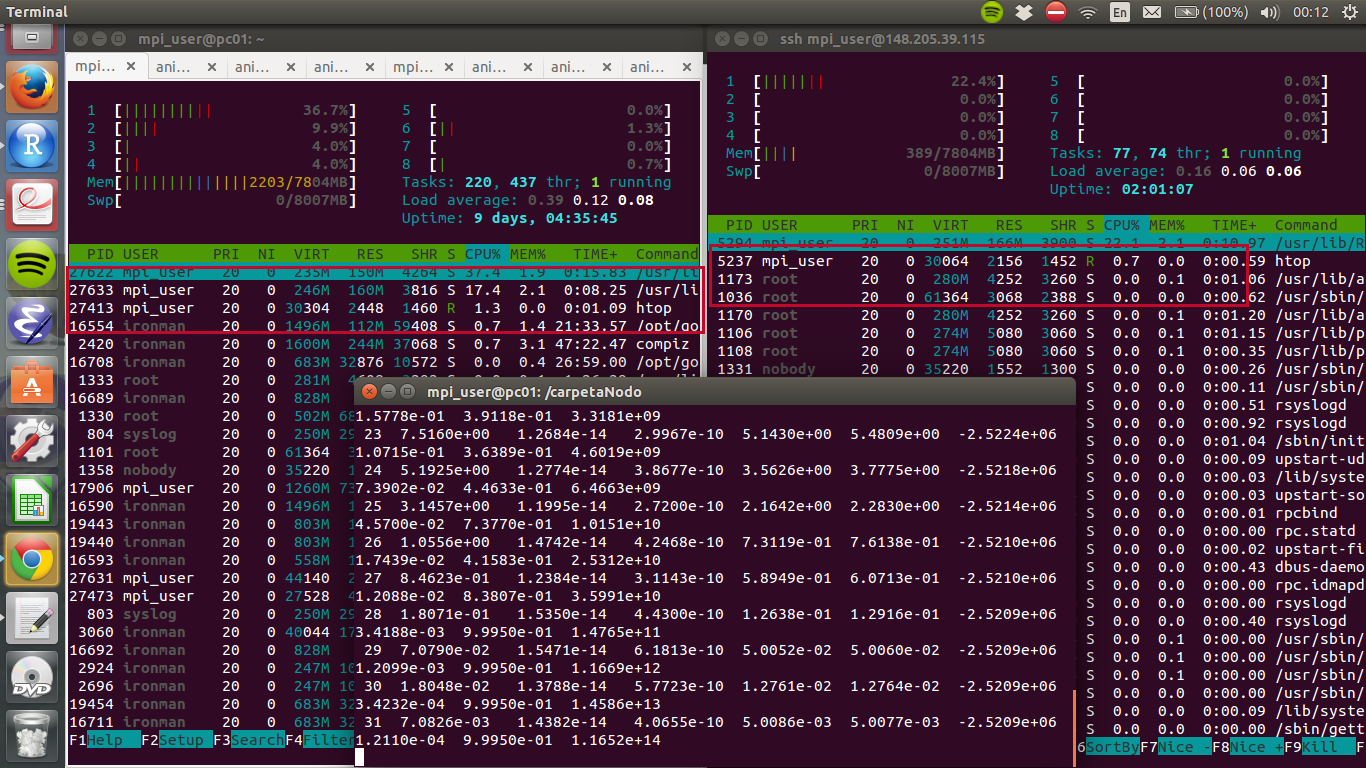
\includegraphics[width=0.8\textwidth]{img/paralelo.png}
\caption{Revisión del proceso en los esclavos y en master.}

\end{figure}

\end{document}
